\chapter{Fonctionnement général}
\begin{figure}[H]
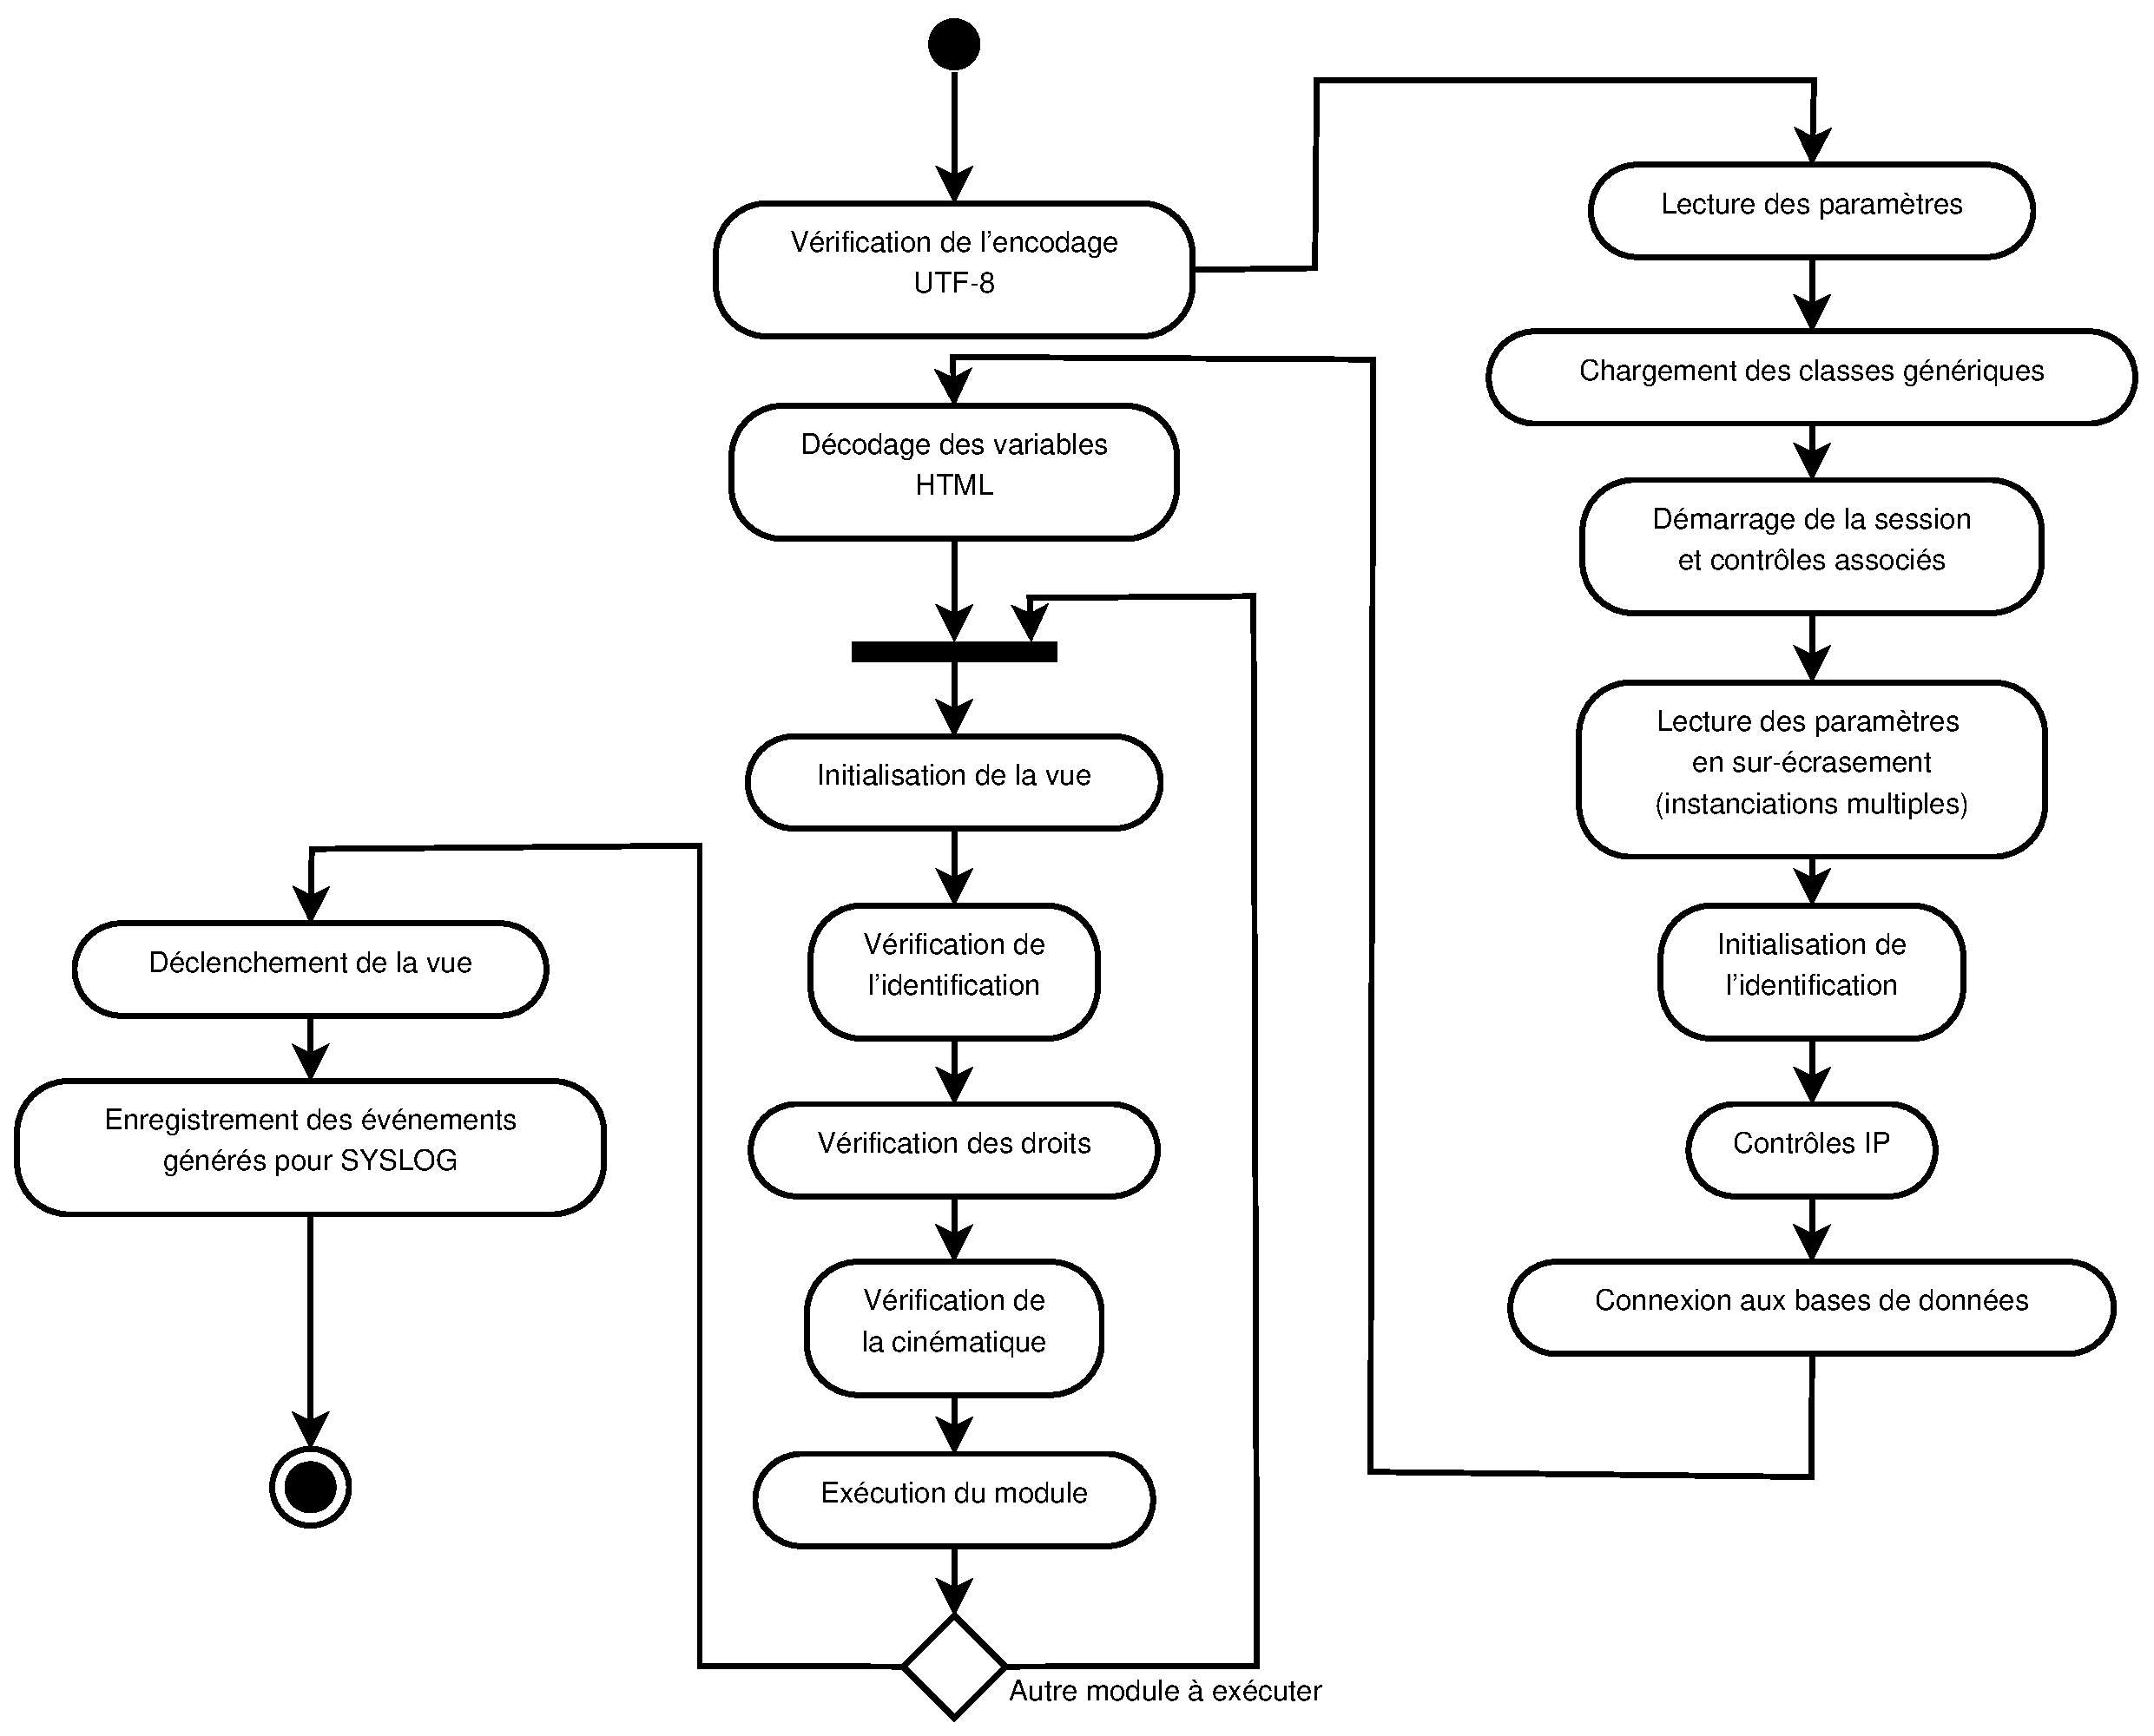
\includegraphics[width=\linewidth]{dessin/synopsis}
\caption{Synopsis général de fonctionnement du contrôleur}
\end{figure}



\section{Synopsis}

L'appel de toute page dans l'application passe nécessairement par l'ensemble de ces étapes :
\begin{itemize}
\item vérification que l'encodage des caractères transmis respecte bien l'encodage utf-8
\item lecture des paramètres
\item chargement des classes génériques utilisées systématiquement
\item démarrage de la session, et ajout de contrôles (durée de la session ouverte...)
\item lecture des paramètres en sur-écrasement, ce qui permet des implémentations multiples avec le même code
\item initialisation de l'identification
\item contrôles de cohérence IP (vérification que, pour une même session, l'adresse IP ne change pas)
\item lancement des connexions aux bases de données (par défaut, deux connexions : une pour la base des droits, l'autre pour les données applicatives)
\item décodage des variables HTML encodées (protection contre les attaques de type XSS)
\item vérification que la base de données soit bien dans la bonne version
\item vérification que l'appel n'est pas trop rapide (une seconde minimum entre deux appels, sauf requêtes ajax), et temporisation de 30" sinon
\item traitement du module demandé :
\begin{itemize}
\item initialisation, le cas échéant, de la vue associée 
\item vérification de l'identification, ou déclenchement des procédures d'identification
\item vérification des droits nécessaires pour accéder au module, et envoi d'un mail aux administrateurs en cas de problème
\item vérification, le cas échéant, de la cinématique : les opérations de modification ne devraient être possibles que si l'opération précédente correspond à l'affichage du formulaire de saisie
\item le cas échéant, vérification du nombre d'appels du module sur la dernière heure ou pour les 10 dernières heures, et blocage si le nombre défini initialement est atteint, avec envoi d'un mail aux administrateurs
\item exécution du module
\item analyse du code de retour du module, et enchaînement le cas échéant sur un autre module
\end{itemize}
\item déclenchement de la vue 
\item enregistrement, le cas échéant, des messages destinés à SYSLOG (messages systèmes)
\end{itemize}

\section{Organisation des dossiers}
Les fichiers sont organisés selon cette arborescence :
\begin{itemize}
\item \textbf{database} : dossier de travail contenant la description de la base de données, la documentation pour les développeurs, les scripts. Le dossier doit être supprimé lors de la mise en production
\item \textbf{display} : le seul dossier accessible. Il contient tous les fichiers nécessaires pour gérer l'affichage :
\begin{itemize}
\item \textbf{bower\_components} : les bibliothèques Javascript installées automatiquement
\item \textbf{CSS} : les feuilles de style
\item \textbf{images} : les icônes et images utilisées dans l'affichage des pages
\item \textbf{javascript} : l'ensemble des librairies Javascript utilisées
\item \textbf{templates} : les modèles de documents utilisés par Smarty (cf. \ref{smarty}, \textit{\nameref{smarty}}, page \pageref{smarty})
\item \textbf{templates\_c} : dossier utilisé par Smarty pour compiler les templates. Ce dossier doit être accessible en écriture par le serveur Web
\end{itemize}
\item \textbf{doc} : ancien dossier, contenant un mécanisme de gestion de la documentation en ligne. N'est plus utilisé actuellement, mais pourrait être employé le cas échéant
\item \textbf{framework} : le code de base du framework. Il comprend :
\begin{itemize}
\item \textbf{dbparam} : dossier permettant de gérer les paramètres stockés en base de données
\item \textbf{dbversion} : dossier permettant de vérifier la version de la base de données
\item \textbf{documentation} : la documentation pour les utilisateurs décrivant certaines fonctionnalités du framework
\item \textbf{droits} : dossier permettant de gérer les droits 
\item \textbf{identification} : gestion de la connexion des utilisateurs
\item \textbf{import/import.class.php} : classe créée il y a quelques années pour gérer les imports (obsolète en grande partie)
\item \textbf{ldap/ldap.class.php} : connexion à un annuaire LDAP et récupération d'informations
\item \textbf{log} : gestion des traces enregistrées dans la base de données
\item \textbf{navigation} : programmes utilisés pour générer le menu et décoder les actions demandées à partir du fichier XML les contenant
\item \textbf{objetbdd} : dossier contenant la classe d'accès aux données de la base de données
\item \textbf{translateId/translateId.class.php} : classe permettant de transcoder les identifiants des enregistrements de la base de données, pour éviter les attaques par forçage de clé
\item \textbf{upgrade} : consignes de mise à jour du framework
\item \textbf{utils} : utilitaires, permettant notamment d'afficher la structure de la base de données
\item de nombreux fichiers utilisés par le framework, dont le contrôleur (controller.php), des fonctions génériques (fonctions.php)...
\item \textbf{vue.class.php} : les classes utilisées pour les vues (cf. \ref{vue} \textit{\nameref{vue}}, page \pageref{vue})
\end{itemize}
\item \textbf{install} : contient des scripts d'installation de la base de données
\item \textbf{locales} : dossier contenant les fichiers de langue
\item \textbf{modules} : dossier contenant le code spécifique de l'application. Il est organisé ainsi :
\begin{itemize}
\item \textbf{classes} : les classes nécessaires pour l'application
\item \textbf{example} : des exemples de codage
\item les autres dossiers sont libres et contiennent les modules de l'application
\item \textbf{beforeDisplay.php} : fichier appelé systématiquement avant l'affichage des pages HTML
\item \textbf{beforesession.inc.php} : fichier appelé systématiquement avant le démarrage de la session. Il permet de déclarer les librairies qui sont nécessaires pour instancier des classes stockées en variables de session
\item \textbf{common.inc.php} : fichier appelé systématiquement avant le traitement des modules
\item \textbf{fonctions.php} : fonctions déclarées par le programmeur et disponibles dans toute l'application 
\item \textbf{postLogin.php} : script exécuté uniquement après qu'un utilisateur se soit identifié
\end{itemize}
\item \textbf{param} : dossier contenant les paramètres de l'application :
\begin{itemize}
\item \textbf{actions.xml} : fichier contenant la description de l'ensemble des modules utilisables, avec les droits associés et le type de vue à utiliser
\item \textbf{menu.xml} : description du menu qui sera généré
\item \textbf{param.default.inc.php} : les paramètres par défaut
\item \textbf{param.inc.php} : paramètres en écrasement, spécifiques de l'implémentation. Ce fichier n'est jamais livré lors des mises à jour, pour éviter la suppression des paramètres de base de données, par exemple
\item \textbf{param.inc.php.dist} : fichier d'exemple de \textit{param.inc.php}, à renommer et à mettre à jour lors de l'installation d'une nouvelle implémentation
\end{itemize}
\item \textbf{plugins} : dossier contenant les bibliothèques PHP tierces non installées automatiquement par \textit{composer}
\item \textbf{temp} : dossier de stockage temporaire, qui doit être accessible en écriture au serveur web. Les fichiers présents dans celui-ci ont une durée de vie de 24 heures (suppression lors de la connexion d'un utilisateur)
\item \textbf{test} : dossier utilisé pour réaliser certains tests. Doit être systématiquement supprimé lors de la mise en production
\end{itemize}

Seuls le fichier \textit{index.php}, à la racine, les dossiers \textit{display} et \textit{test} sont accessibles directement. Les autres dossiers sont protégés par des fichiers \textit{.htaccess}.

\section{Paramètres}\label{param}

Les paramètres utilisés dans l'application sont gérés avec 3 fichiers différents :
\begin{itemize}
\item \textbf{param/param.default.inc.php} : contient l'ensemble des paramètres utilisés ;
\item \textbf{param/param.inc.php} : contient ceux issus du fichier précédent, qui sont adaptés à l'implémentation ;
\item \textbf{param.ini} : fichier contenant les paramètres spécifiques du nom DNS de l'application (par exemple, schéma particulier associé au nom du site). Pour plus d'informations sur ce point, consultez le chapitre \ref{dnsmultiple} \textit{\nameref{dnsmultiple}}, page \pageref{dnsmultiple}.
\end{itemize}

Voici la description de l'ensemble des paramètres :

\subsection{Paramètres généraux}
% \usepackage{array} is required
\begin{longtable}{|p{5cm}|p{8cm}|}
\hline
\textbf{Variable} & \textbf{Signification} \\
\hline
\endhead
\hline
\endfoot\endlastfoot
APPLI\_version & Numéro de version de l'application \\ 

APPLI\_versiondate & Date de la version \\ 

language & Langue par défaut \\

DEFAULT\_formatdate & Format par défaut d'affichage des dates\\

navigationxml & nom du fichier XML contenant la description des modules exécutables\\

APPLI\_session\_ttl & durée de la session, en secondes\\

APPLI\_cookie\_ttl & durée de vie par défaut des cookies, en secondes\\

LOG\_duree & Durée de conservation des traces des actions réalisées, en jours\\

APPLI\_mail & Adresse pour déclarer les incidents (mail ou non)\\

APPLI\_titre & Nom de l'application qui sera affiché (cas où le code est utilisé par plusieurs entrées différentes) \\

APPLI\_code & Code interne de l'application. Utilisé dans certains cas\\

APPLI\_fds & Feuille de style utilisée par défaut (obsolète)\\

APPLI\_address & Adresse DNS de l'application. Utilisée en cas d'identification CAS (adresse de retour)\\

APPLI\_modeDeveloppement & si à true, certaines opérations sont réalisées dans un contexte de développement (affichage de messages, recalcul systématique du menu...)\\

APPLI\_notSSL & utilisé en développement, si l'application ne fonctionne pas en mode SSL (déconseillé) \\

APPLI\_utf8 & systématiquement à true (plus de support des autres encodages)\\

APPLI\_menufile & nom du fichier XML contenant la description du menu\\

APPLI\_temp & nom du dossier utilisé pour stocker les fichiers temporaires\\

APPLI\_moduleDroitKO & nom du module appelé en cas de refus d'accès pour un problème de droits \\

APPLI\_moduleErrorBefore & nom du module appelé en cas de problème lié à la cinématique de l'application\\

APPLI\_moduleNoLogin & nom du module appelé en cas d'échec d'identification \\

APPLI\_passwordMinLength  & Longueur minimale du mot de passe \\
APPLI\_hour\_duration  & Duration of an hour for count all calls to a module\\
APPLI\_day\_duration  & Duration of a day for count all calls to a module \\
MAIL\_enabled & Autorise l'envoi de mails \\
APPLI\_delay\_between\_call & delay between call of modules others than ajax \\
APPLI\_sleep\_duration  & durée de temporisation si des requêtes sont trop rapprochées (\textit{cf.} APPLI\_delay\_between\_call) \\

paramIniFile & nom du fichier contenant les paramètres spécifiques liés au DNS utilisé (\textit{cf.} \ref{dnsmultiple} \textit{\nameref{dnsmultiple}}, page \pageref{dnsmultiple}) \\

SMARTY\_param & Paramètres utilisés par le moteur de templates SMARTY\\

SMARTY\_variables & variables systématiquement transmises à SMARTY et utilisées lors de l'affichage général\\

ERROR\_display & Affiche les erreurs à l'écran (mode développement)\\

OBJETBDD\_debugmode & 0 : pas d'affichage de message d'erreur, 1, affichage des messages d'erreur, 2 : affichage de toutes les commandes SQL générées par ObjetBDD \\
\hline

\caption{Variables générales de l'application}
\end{longtable} 

\subsection{Identification}\label{paramident}
\begin{longtable}{|p{5cm}|p{8cm}|}
\hline
\textbf{Variable} & \textbf{Signification} \\
\hline
\endhead
\hline
\endfoot
\endlastfoot
ident\_type & Type d'identification supporté. L'application peut gérer \textbf{BDD} (uniquement en base de données),\textbf{LDAP} (uniquement à partir d'un annuaire LDAP) \textbf{LDAP-BDD} (d'abord identification en annuaire LDAP, puis en base de données), \textbf{CAS} (serveur d'identification \textit{Common Access Service}), et enfin \textbf{HEADER} (identification derrière un proxy qui fournit le login dans une variable d'entête HTTP ou \textit{via} une identification Shibboleth)\\
CAS\_plugin & Nom du plugin utilisé pour une connexion CAS \\
CAS\_address & Adresse du serveur CAS\\
CAS\_port & Systématiquement 443 (connexion chiffrée)\\
CAS\_debug & Activation du mode debug \\
CAS\_CApath & Chemin d'accès au certificat du serveur CAS \\
LDAP & tableau contenant tous les paramètres nécessaires pour une identification LDAP \\
ident\_header\_login\_var & par défaut, AUTH\_USER. Nom de la variable qui contiendra le login dans le cas d'une identification en mode HEADER (le radical HTTP\_  ne doit pas être indiqué) \\

privateKey & clé privée utilisée pour générer les jetons d'identification \\

pubKey & clé publique utilisée pour générer les jetons d'identification \\

tokenIdentityValidity & durée de validité, en secondes, des jetons d'identification\\

MAIL\_enabled & si à 1, l'envoi de mail est géré par l'application \\

CONNEXION\_max\_attemps & nombre maximum d'essais de connexion avant blocage du compte \\

CONNEXION\_blocking\_ duration & durée de blocage du compte \\

APPLI\_mailToAdminPeriod & durée minimale d'envoi d'un mail de signalement d'un problème aux administrateurs (pour éviter une saturation de boite) \\

APPLI\_admin\_ttl & durée, en secondes, de la durée de vie de la session d'administration (accès aux modules de droit admin). Au delà, l'administrateur doit se ré-authentifier \\

APPLI\_lostPassword & Si à 1, autorise la récupération du mot de passe perdu (nécessite également que le paramètre MAIL\_enabled soit positionné à 1) \\
\hline

\caption{Variables utilisées pour paramétrer l'identification}
\end{longtable}

Voici le contenu des variables du tableau LDAP : 
\begin{longtable}{|p{5cm}|p{8cm}|}
\hline
\textbf{Variable} & \textbf{Signification} \\
\hline
\endhead
address &  adresse de l'annuaire\\
port & 389 en mode non chiffré, 636 en mode chiffré\\
rdn & compte de connexion, si nécessaire \\
basedn & base de recherche des utilisateurs\\
user\_attrib & nom du champ contenant le login à tester\\
v3 & toujours à \textit{true}\\
tls & \textit{true} en mode chiffré\\
groupSupport & \textit{true} si l'application recherche les groupes d'appartenance du login dans l'annuaire\\
groupAttrib & Nom de l'attribut contenant la liste des groupes d'appartenance\\
commonNameAttrib & Nom de l'attribut contenant le nom de l'utilisateur\\
mailAttrib & Nom de l'attribut contenant l'adresse mail de l'utilisateur\\
attributgroupname & Attribut contenant le nom du groupe lors de la recherche des groupes (cn par défaut)\\
attributloginname & attribut contenant les membres d'un groupe\\
basedngroup & base de recherche des groupes \\
timeout & délai, en secondes, du timeout d'accès à l'annuaire \\
\hline
\caption{Variables utilisées pour paramétrer l'accès à l'annuaire LDAP}
\end{longtable}

Variables transmises systématiquement à Smarty pour affichage dans toutes les pages :

\begin{longtable}{|p{5cm}|p{8cm}|}
\hline
\textbf{Variable} & \textbf{Signification} \\
\hline
\endhead
entete & nom du template contenant le haut de la page et le menu \\
enpied & nom du template contenant le pied de page \\
corps & nom du template contenant le corps de la page (mis à jour dans chaque module d'affichage)\\
melappli & mail générique de l'application, utilisé lors de l'envoi de messages \\
ident\_type & mode d'identification utilisé \\
appliAssist & adresse du site d'assistance ou de dépôt de ticket \\
\hline
\caption{Variables transmises en tableau à Smarty systématiquement pour l'affichage dans toutes les pages}
\end{longtable}


\subsection{Connexions aux bases de données}

Deux connexions sont systématiquement implémentées : l'une à la base de données contenant la gestion des droits, et l'autre à celle contenant les données propres à l'application.
\begin{longtable}{|p{5cm}|p{8cm}|}
\hline
\textbf{Variable} & \textbf{Signification} \\
\hline
\endhead
\hline\endfoot\endlastfoot
BDD\_login & compte de connexion à la base de données \\
BDD\_passwd & mot de passe associé\\
BDD\_dsn & adresse de la base de données sous forme normalisée\\
BDD\_schema & schéma utilisé (plusieurs schémas peuvent être décrits, en les séparant par une virgule - fonctionnement propre à Postgresql)\\
GACL\_dblogin & compte de connexion à la base de données des droits\\
GACL\_dbpasswd & mot de passe associé\\
GACL\_dsn & adresse normalisée \\
GACL\_schema & schéma utilisé\\
GACL\_aco & nom du code de l'application utilisé dans la gestion des droits (\textit{cf.} \ref{droits} \textit{\nameref{droits}}, page \pageref{droits} )\\

\hline
\caption{Variables utilisées pour paramétrer les connexions}
\end{longtable}

Il est possible de créer des comptes séparés, voire de ne donner accès qu'en lecture à la base des droits (à l'exception de la table \textit{log}, qui contient la trace de toutes les actions demandées).

\section{Gestion des messages}

Une classe est instanciée systématiquement pour gérer les messages, la classe \textit{Message}. Deux types de messages sont pris en compte :
\begin{itemize}
\item les messages envoyés au navigateur, à destination de l'utilisateur ;
\item les messages enregistrés dans Syslog, le mécanisme de gestion des messages systèmes de Linux.
\end{itemize}

Les messages sont enregistrés dans un tableau, qui sera ensuite dépilé pour générer les textes soit à afficher, soit à stocker dans Syslog.

La classe dispose des fonctions suivantes :
\begin{longtable}{|p{5cm}|p{8cm}|}
\hline
\textbf{fonction} & \textbf{Objectif} \\
\hline
\endhead
\hline\endfoot\endlastfoot
\_\_construct(\$displaySyslog = false) & Constructeur de la classe. La variable permet d'indiquer si les messages destinés à Syslog sont également affichés à l'écran (mode par défaut en développement) \\
set(\$value) & Ajoute un nouveau libellé pour utilisateur \\
setSyslog(\$value) & Ajout un nouveau message système \\
get() & Retourne le tableau contenant l'ensemble des messages, avec ou sans les messages systèmes, selon le mode indiqué dans le constructeur \\
getAsHtml() & Formate les messages pour les envoyer au navigateur. Chaque message est séparé par un retour à la ligne. Les libellés sont encodés en HTML avant d'être envoyés \\
sendSyslog() & Génère un message dans Syslog. Actuellement, le message est toujours de type NOTICE. \\
\hline

\caption{Fonctions utilisables dans la classe Message}
\end{longtable}

Les messages sont systématiquement transmis à la vue Smarty, et l'envoi des messages systèmes est la dernière action réalisée avant l'affichage de la vue.

\chapter{Décrire les actions}\label{labelxml}

Les actions possibles dans le logiciel sont décrites dans un fichier, par défaut \textit{param/actions.xml}. C'est un fichier XML dont la racine s'appelle \textit{navigation}. 

Une action est la conjonction entre un contexte et une opération, par exemple \textit{poissonList} pour afficher la liste des poissons, \textit{poissonChange} pour afficher la page de modification d'un poisson, \textit{poissonWrite} ou \textit{poissonDelete} pour déclencher l'écriture en base de données.

Dans le contexte de ce framework, l'action s'appelle \textit{module} (nom du champ transmis depuis le navigateur). L'attribut \textit{action} contient le nom du fichier PHP appelé. Il est associé à l'attribut \textit{param}, qui permet d'indiquer le détail de l'action à réaliser (par exemple, \textit{list} ou \textit{change}).

Voici la liste des attributs disponibles pour un module (ou une action) :
\begin{longtable}{|p{2.5cm}|c|p{9cm}|}
\hline
\textbf{Attribut} & \textbf{Requis} & \textbf{Signification} \\
\hline
\endhead
\hline\endfoot\endlastfoot
action & X & nom de la page PHP à exécuter (accès relatif depuis la racine de l'application) \\
param &  & paramètre analysé dans la page, pour savoir quelle action doit être réalisée. Par convention, les actions possibles sont les suivantes : list, read, change, write, delete, ou autre action \\
droits &  & Liste des droits nécessaires pour exécuter l'action. Si plusieurs droits sont possibles, ils doivent être séparés par une virgule\\
loginrequis & & Indique, en l'absence de droits spécifiques, si l'action nécessite d'être connecté. Vaut 1 si la connexion est requise\\
modulebefore & & Pour les opérations d'écriture, permet d'indiquer le nom du module qui doit impérativement être exécuté avant. Cela limite les risques d'attaques de type CSRF et les rafraîchissements intempestifs dans les formulaires. Plusieurs modules peuvent être indiqués, en les séparant par une virgule\\
retourok & & indique le nom du module qui sera exécuté si le code de retour (variable \$module\_coderetour) vaut 1 \\
retourko & & indique le nom du module qui sera exécuté si le code de retour (variable \$module\_coderetour) vaut -1 (échec d'exécution) \\
type & (X) & pour les modules envoyant des données au navigateur, indique le type de la vue qui sera utilisée. Les valeurs possibles sont smarty ou html (même vue), ajax, pdf, csv, binaire (pour les images), file (pour envoyer un fichier directement)  \\
droitko & & nom du module appelé si les droits ne sont pas suffisants pour exécuter l'action demandée \\
maxCountBy Hour & & nombre d'appels au module possibles par heure (login/ip) \\
maxCountBy Day & & nombre d'appels au module possibles par jour (login/ip) \\
\hline 
 
 \caption{Liste des attributs utilisables pour décrire une action}\label{actions}
\end{longtable}

Le module \textit{model} n'est pas analysé, il sert à montrer l'ensemble des options possibles. 

Le module \textit{default} correspond au module appelé par défaut, si l'application est appelée sans indiquer de nom de module (variable \textit{module} non transmise soit dans le lien, soit dans le formulaire).

Voici quelques exemples d'utilisation :
\begin{lstlisting}
	<appliList action="framework/droits/appli.php" param="list" droits="admin" retourlogin="1"  type="smarty" />
	<appliDisplay action="framework/droits/appli.php" param="display" droits="admin"  type="smarty"/>
	<appliChange action="framework/droits/appli.php" param="change" droits="admin"  type="smarty"/>
	<appliWrite action="framework/droits/appli.php" param="write" droits="admin" retourok="appliDisplay" retourko="appliChange" modulebefore="appliChange" />
	<appliDelete action="framework/droits/appli.php" param="delete" droits="admin" retourok="appliList" retourko="appliChange"  modulebefore="appliChange"/>
\end{lstlisting}

Il s'agit des modules utilisés dans la gestion des droits. Ils nécessitent tous que l'utilisateur dispose du droit \textit{admin}. Une seule page est appelée (\textit{appli.php}), l'action à réaliser étant analysée à partir de l'attribut \textit{param}.

Les modules \textit{appliWrite} et \textit{appliDelete} ne génèrent pas directement d'affichage : ils sont là uniquement pour écrire des informations dans la base de données. Par contre, ils enchaînent, en fonction de leur code de retour, soit sur le réaffichage du formulaire de saisie, soit sur le retour au détail ou à la liste.
Ces deux modules ne peuvent être exécutés que si le précédent est \textit{appliChange}, c'est à dire si le formulaire de saisie a été affiché.

\chapter{Identifier les utilisateurs et gérer les droits}\label{droits}
\section{Identifier les utilisateurs}

Cinq modes d'identification sont prévus dans le logiciel :
\begin{itemize}
\item uniquement dans le logiciel (comptes stockés dans la base de données) ;
\item à partir d'un annuaire LDAP ;
\item d'abord en recherchant dans l'annuaire LDAP, puis ensuite dans la base des comptes de l'application (mode mixte) ;
\item auprès d'un serveur CAS ;
\item derrière un serveur d'identification, type LemonLdap\footnote{LemonLdap (\url{http://lemonldap-ng.org}) est un serveur proxy qui s'interface entre l'utilisateur et le serveur web de l'application. Il gère l'identification des utilisateurs, et n'autorise l'accès au serveur web applicatif que si elle est réussie}, qui fournit l'identification dans une variable HEADER. Ce mode est compatible avec l'identification Shibboleth, configurée avec le mode Apache Mellon.
\end{itemize}

L'identification retenue est déclarée dans les paramètres généraux (\textit{cf.} \ref{paramident} \textit{\nameref{paramident}}, page \pageref{paramident}).

Si l'identification à partir d'un annuaire LDAP ou d'un serveur CAS ne nécessite guère d'autres informations que celles décrites dans les paramètres, l'identification par base de données comprend des mécanismes particuliers pour protéger les mots de passe et limiter les risques associés. Voici les règles imposées lors de la création d'un mot de passe : 
\begin{itemize}
\item il doit avoir une longueur minimale de 12 caractères (paramétrable) ;
\item il doit comporter 3 jeux de caractères différents (minuscules, majuscules, chiffres et autres caractères) ;
\item il ne doit pas être trop commun (contrôle de complexité avec une bibliothèque externe)
\end{itemize}

Les mots de passe sont stockés au format bcrypt depuis juillet 2019. Les anciens mots de passe (chiffrement AES256 avec sel) sont toujours reconnus.

L'écran de création propose un bouton de génération automatique d'un mot de passe, qui devra être transmis à l'utilisateur, en lui demandant d'en changer (il peut modifier son mot de passe une fois connecté). Il ne pourra se connecter que 3 fois avec ce mot de passe : il devra le modifier rapidement.

Le framework dispose d'un mécanisme de récupération par envoi de mails, avec génération d'un jeton à usage unique.

Hormis pour les mots de passe générés par l'administrateur, les mots de passe n'expirent pas.

\subsection{Identification par HEADER}

Dans ce mode d'identification, le serveur web est placé derrière un serveur d'identification, appelé proxy d'identification. L'adresse de l'application pointe vers ce dernier. 

Le proxy gère la connexion de l'utilisateur, et fournit à l'application le login dans une variable configurable. Cette variable est accessible dans le tableau \$\_SERVER, par exemple \$\_SERVER["HTTP\_AUTH\_USER"].

Pour activer ce mécanisme, il faut modifier les paramètres suivants dans le fichier \textit{param.ini.php} (\textit{cf.} \ref{paramident} \textit{\nameref{paramident}}, page \pageref{paramident})\footnote{Le mode HEADER n'a encore jamais été testé (version 3.0.0 du \textit{framework})} :
\begin{lstlisting}
$ident_type = "HEADER";
$ident_header_login_var = "AUTH_USER";
\end{lstlisting}

la variable ne doit pas contenir la racine HTTP\_ (une fonction l'extrait automatiquement).

\subsection{Ré-identification par jeton}

Par défaut, les sessions ont une durée de vie d'une heure. Dans certains cas de figure, il est souhaitable que l'utilisateur n'ait pas à ressaisir ses identifiants systématiquement.

Le framework peut générer un jeton chiffré après la première identification, qui sera analysé pour savoir si l'utilisateur peut être ré-identifié automatiquement.

Pour que ce mécanisme fonctionne, il faut :
\begin{itemize}
\item que le paramètre \textit{tokenIdentityValidity} ait une durée de validité supérieure à la durée de vie de la session. Il est raisonnable de ne pas fixer une durée de vie supérieure à une journée de travail (10 heures). Le cookie transmis est protégé ;
\item que les clés privée et publique, utilisées pour le chiffrement du jeton, soient accessibles au serveur web (variables \textit{privateKey} et \textit{publicKey}).
\end{itemize}

Le jeton est chiffré avec la clé privée, ce qui lui permet d'être lu, le cas échéant, par l'application. Il contient le login, la date d'expiration et l'IP du poste de l'utilisateur. 

Si l'utilisateur déclenche une déconnexion, le jeton est supprimé.

\subsection{Support de la double authentification via TOTP}

Les utilisateurs ont la possibilité d'activer la double identification en utilisant le protocole TOTP. Cette double identification est compatible avec tous les modes (non testé au 22/02/2021 avec le mode HEADER et le mode Mellon).

Les clés secrètes sont stockées dans la table gacl.acllogin, et sont chiffrées avec la clé publique utilisée pour générer les jetons de réidentification. 

Pour désactiver la double authentification, il faut modifier la fiche correspondante dans l'application (ACL - logins).

\subsection{Support du mode Shibboleth avec Mellon}

L’identification est réalisée en utilisant un module Apache dédié : Mellon \linebreak (\href{https://github.com/latchset/mod_auth_mellon}{https://github.com/latchset/mod\_auth\_mellon}).

Elle nécessite de récupérer les informations techniques liées à la fédération, et d’enregistrer l’application chez le fournisseur de l’identification.

\subsubsection{Installation du module Mellon}

\begin{lstlisting}
apt-get install libapache2-mod-auth-mellon
\end{lstlisting}


Si le paquet libapache2-mod-auth-mellon n’est pas disponible (cas rencontré avec une distribution Debian strech), vous devrez récupérer et installer les paquets suivants (dans l’ordre) :
\begin{itemize}
	\item libxmlsec1
	\item libxmlsec1-openssl
	\item liblasso3
	\item libapache2-mod-auth-mellon
\end{itemize}
    
  
Vous devrez également récupérer le fichier xml de votre provider, ainsi que son certificat.

\subsubsection{Génération des fichiers de configuration de l’application}

Un certificat (et sa clé privée), un fichier xml doivent être générés pour l’application. Un script est disponible dans les distributions Debian. Il est également fourni dans l’application, dans le dossier install/apache2 (create\_metadata.sh).

Pour générer les fichiers (remplacez collec-science.com par vos propres valeurs) :

\begin{lstlisting}
cd /etc/apache2
mkdir mellon
cd mellon
/var/www/html/collec-science/collec/install/apache2/create_metadata.sh https://collec-science.com https://collec-science.com/mellon
\end{lstlisting}

Le certificat (fichier .cert) et le fichier xml doivent être transmis au provider, pour qu’il les intègre dans sa plate-forme. Vous devez également récupérer du provider sa clé publique et son certificat d’autorité racine, à mettre dans le dossier mellon. Il doit également vous fournir un fichier xml qui contient les adresses de toutes les entités participant à la fédération.

\subsubsection{Configurer le site virtuel}

Recopiez le fichier \textit{install/apache2/prototypephp-mellon.conf} dans le dossier \textit{/etc/apache2/sites-available}, à la place du fichier prototypephp.conf. Éditez le fichier, et remplacez toutes les chaînes collec.mysociety.com par votre DNS. Vérifiez également les certificats utilisés.

Par rapport au fichier classique, le fichier prototypephp-mellon.conf contient, dans la section <VirtualHost *443>, les commandes suivantes :

\begin{lstlisting}
# Configuration Mellon for Renater
<location />
AuthType Mellon
MellonEnable "auth"
MellonSecureCookie On
MellonUser MAIL
MellonMergeEnvVars On
MellonSubjectConfirmationDataAddressCheck Off
MellonSPPrivateKeyFile /etc/apache2/mellon/https_collec.mysociety.com.key
MellonSPCertFile /etc/apache2/mellon/https_collec.mysociety.com.cert
MellonSPentityId "https://collec.mysociety.com"
MellonSPMetadataFile "/etc/apache2/mellon/https_collec.mysociety.com.xml"
MellonIdPMetadataFile "/etc/apache2/mellon/main-idps-renater-metadata.xml"
MellonIdPPublicKeyFile "/etc/apache2/mellon/renater-metadata-signing-cert-2016.pem"
MellonIdPCAFile "/etc/apache2/mellon/renater-metadata-signing-cert-2016.pem"
MellonProbeDiscoveryTimeout 1
MellonSetEnv "MAIL" "urn:oid:0.9.2342.19200300.100.1.3"
MellonSetEnv "GIVENNAME" "urn:oid:2.5.4.42"
MellonEndpointPath /mellon
MellonSetEnvNoPrefix REMOTE_USER NAME_ID
MellonDiscoveryURL "https://discovery.renater.fr/renater/WAYF"
</location>
\end{lstlisting}

Les rubriques \textit{MellonIdP*} doivent être adaptées aux fichiers fournis par votre provider.

Une fois la configuration effectuée, redémarrez le serveur Apache :

\begin{lstlisting}
systemctl restart apache2
\end{lstlisting}


\subsubsection{Enregistrer le site dans la fédération Renater}

Pour les établissements français affiliés à la fédération Renater, vous pouvez enregistrer directement votre application dans celle-ci. Des validations seront réalisées par les contacts de la fédération dans votre établissement.

Pour réaliser l’enregistrement :
\begin{itemize}
	\item Connectez-vous au site \href{https://registry.federation.renater.fr/}{https://registry.federation.renater.fr/}
	\item cliquez sur Ajouter un fournisseur de services
	\item dans l’onglet Description, renseignez les champs demandés, avec notamment :
	\begin{itemize}
		\item URL du service : https ://collec.mysociety.com (votre DNS)
	\end{itemize}
	\item dans l’onglet Contacts, ne vous déclarez pas conforme au cadre de sécurité SIRTFI, sauf si vous savez ce que c’est (il y a des contraintes organisationnelles fortes pour être conforme)
	\item dans l’onglet Attributs demandés, demandez les attributs :
	\begin{itemize}
		\item email : identification des utilisateurs (obligatoire)
		\item commonName : affichage du nom des utilisateurs (obligatoire)
	\end{itemize}
	\item dans l’onglet Informations techniques, indiquez l’adresse suivante pour récupérer les données de configuration :
	\begin{itemize}
		\item URL de vos métadonnées : https ://collec.mysociety.com/mellon/metadata
	\end{itemize}
\end{itemize}

Une fois le dossier validé, vous devrez attendre le retour de votre correspondant Renater dans votre établissement, qui doit valider votre demande.
Une fois cette première demande réalisée, vous devrez vous reconnecter au site de la fédération, et activer le rattachement à la fédération choisie (onglet Rattachement à une fédération). Deux fichiers seront à récupérer (commande \textit{wget} dans le dossier \textit{/etc/apache2/mellon}) pour récupérer d’une part le certificat, et d’autre part le fichier XML contenant l’ensemble des fournisseurs attachés à la fédération.

Ce rattachement doit également être validé par votre correspondant Renater.

Attention : une fois le rattachement validé, vous devrez attendre 24 heures pour que votre application soit disponible auprès de l’ensemble des membres de la fédération, et donc pouvoir vous connecter.

\section{Gérer les droits}

Les droits sont gérés selon le principe initialement utilisé dans la bibliothèque PHPGACL, aujourd'hui obsolète. 

Les logins sont déclarés dans des groupes organisés de manière hiérarchique : un groupe hérite des droits attribués à ses parents.

Les droits utilisés dans le logiciel sont associés à des groupes. Il est possible d'attribuer plusieurs droits à un même groupe, et un droit peut être détenu par des groupes différents.

Si le paramètre \textit{\$LDAP["groupSupport"]} est positionné à \textit{true}, les groupes dont fait partie le compte LDAP sont également récupérés, et peuvent être détenteurs de droits dans le logiciel (le nom des groupes est sensible à la casse).

Voici le schéma des tables utilisées pour gérer les droits :

\begin{figure}[H]
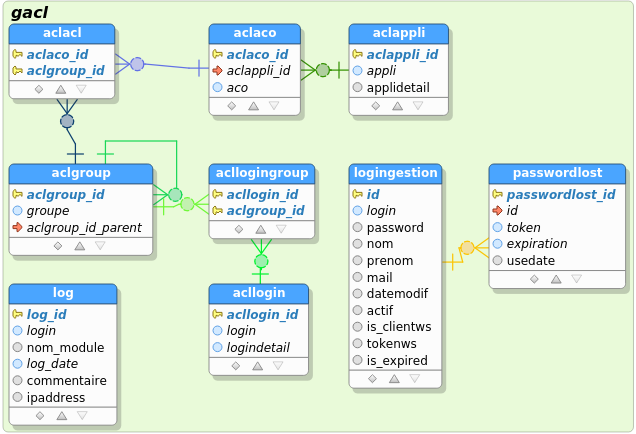
\includegraphics[width=\linewidth]{dessin/gacl}
\caption{Schéma des tables utilisées pour gérer les droits (schéma GACL complet)}
\end{figure}

Voici la description des tables utilisées spécifiquement pour gérer les droits :
\begin{description}
\item[acllogin] Liste des logins utilisés. Si un compte est créé dans la base locale d'identification, un enregistrement est également créé dans cette table. Pour les identifications LDAP ou CAS, ils doivent être identiques. Si seuls les groupes LDAP sont utilisés pour un compte, il n'a pas besoin d'être décrit ici
\item[aclappli] Liste des applications gérées. Il est ainsi possible de gérer, à partir de la même base de données, plusieurs ensembles de droits, qui utilisent les mêmes logins
\item[aclaco] liste des droits déclarés dans l'application
\item[aclgroup] Liste des groupes contenant les logins, et qui détiennent les droits. Un groupe peut hériter d'un autre groupe. Les droits associés au groupe parent sont également attribués au groupe hérité.
\item[acllogingroup] table permettant de déclarer les logins associés à un groupe
\item[aclacl] table décrivant les droits détenus par un groupe
\end{description}

Le module d'administration permet de saisir toutes ces informations. Il faut que l'utilisateur dispose du droit \textit{admin}, c'est à dire faire partie du groupe \textit{admin} (configuration par défaut à l'initialisation de la base des droits) pour pouvoir accéder à ces fonctions.

\subsection{Créer un nouvel utilisateur}

Les utilisateurs peuvent être issus soit de l'annuaire LDAP, soit de la base interne. 
Pour créer un nouvel utilisateur dans la base locale :
\begin{itemize}
\item \textit{Administration $\rightarrow$ Liste des comptes }
\item \textit{Nouveau login}
\item renseignez au minimum le login.
\end{itemize}

\begin{figure}[H]
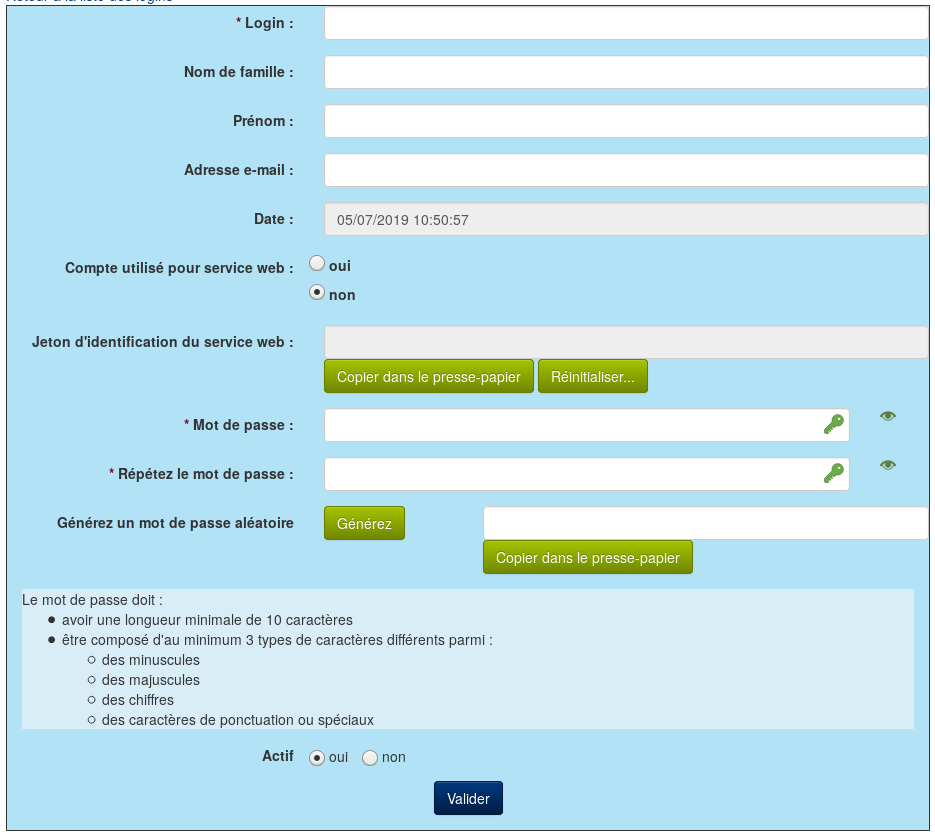
\includegraphics[width=\linewidth]{dessin/creation-login}
\caption{Écran de saisie d'un login de connexion}
\end{figure}

Pour créer le mot de passe, vous pouvez cliquer sur le bouton \textit{Générez}, qui  en créera un automatiquement. Envoyez-le par mél à son destinataire (par \textit{copier-coller}), en lui demandant de le modifier à la première connexion (icône en forme de clé, dans le bandeau, en haut à droite).

Les mots de passe doivent respecter les règles suivantes :
\begin{itemize}
\item ils doivent avoir une longueur minimale de 12 caractères (paramétrable) ;
\item ils doivent comprendre trois types de caractères différents parmi les minuscules, majuscules, chiffres et caractères de ponctuation ;
\item les mots de passe n'expirent pas, sauf ceux générés par l'interface : dans ce cas de figure, ils ne peuvent être utilisés que trois fois.
\end{itemize}

Les mots de passe sont stockés sous forme d'empreinte, calculée en rajoutant un sel\footnote{chaîne de caractère rajoutée au mot de passe -- en général le login ou un identifiant -- qui permet d'éviter que deux mots de passe identiques, associés à deux logins différents, aient la même empreinte} et encodés en SHA256 : ils ne peuvent pas être retrouvés en cas de perte.

L'application n'intègre pas de module permettant de régénérer automatiquement un mot de passe en cas de perte : c'est au responsable applicatif d'en fournir alors un nouveau.

La création d'un compte entraîne la création d'une entrée identique dans la table des \textit{acllogin}, utilisée pour attribuer les droits.

Pour désactiver temporairement un compte, sélectionnez \textit{non} dans la zone \textit{actif}. Si le compte ne doit plus être utilisé, supprimez-le.

Attention : si le compte disposait des droits d'administration, assurez-vous que vous avez toujours un compte disposant des mêmes droits avant la suppression.

\subsection{Créer un login utilisé dans la gestion des droits}

Indépendamment du compte de connexion, qui peut être soit issu de la base interne, soit récupéré auprès d'un annuaire LDAP ou d'un serveur CAS, l'application a besoin de connaître les utilisateurs pour pouvoir leur attribuer des droits.

À partir du menu, choisissez \textit{Administration $\rightarrow$ ACL - logins}.

Vous pouvez modifier un login existant ou en créer un nouveau. Dans ce cas, vous devrez indiquer au minimum le login utilisé (identique à celui qui est employé pour la connexion à l'application : base de données interne, annuaire LDAP, serveur CAS).

\begin{figure}[H]
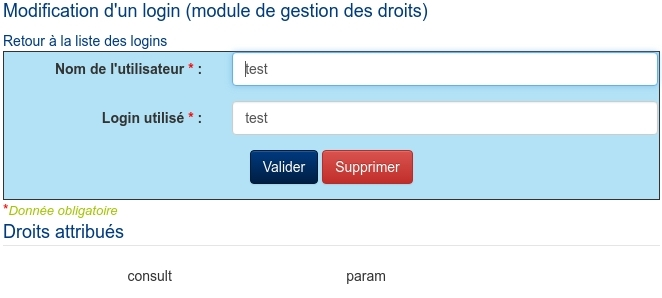
\includegraphics[width=\linewidth]{dessin/acl_login}
\caption{Écran de modification d'un login dans le module de gestion des droits}
\end{figure}


Sous l'écran de saisie figurent la liste des droits attribués à un login (en modification, le calcul n'est réalisé qu'à l'affichage de la page).

\subsection{Définir les groupes d'utilisateur}

Les groupes d'utilisateurs sont gérés selon un mécanisme d'héritage. Un groupe de haut niveau hérite des groupes précédents : si des droits ont été attribués à un groupe de niveau inférieur, un login associé à un groupe de niveau supérieur les récupère également.

Pour définir les groupes, dans le menu, choisissez \textit{Administration $\rightarrow$ ACL - groupes de logins}.

\begin{figure}[H]
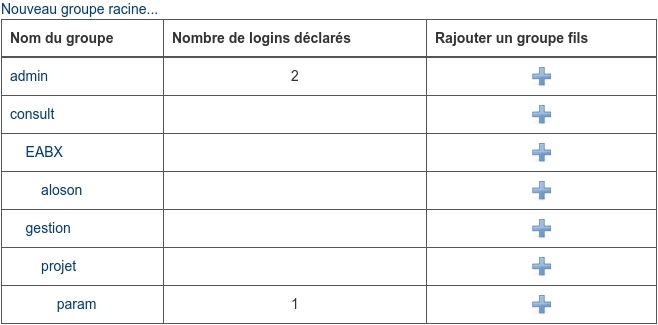
\includegraphics[width=\linewidth]{dessin/acl_groupe}
\caption{Liste des groupes de logins}
\end{figure}

Ainsi, le login déclaré dans le groupe \textit{param} récupérera les droits attribués aux groupes \textit{projet}, \textit{gestion} et \textit{consult}.

Pour créer un groupe, deux possibilités :
\begin{itemize}
\item soit le groupe est à la base d'une nouvelle branche : utilisez alors \textit{Nouveau groupe racine...} ;
\item soit le groupe hérite d'un autre groupe : cliquez sur le signe + (\textit{Rajouter un groupe fils}).
\end{itemize}

Vous pouvez indiquer les logins qui sont rattachés à ce groupe.


\subsection{Créer une application}
Le framework permet de gérer des droits différents pour des jeux de données différents, à partir du même code applicatif. Chaque couple \textit{logiciel} $\leftrightarrow$ \textit{base de données} constitue donc une \textit{application}, au sens de la gestion des droits.

Il est ainsi possible, à partir de la même base de données, de définir des droits différents selon les jeux de données utilisés (un jeu de données correspond à un schéma de base de données comprenant l'intégralité des tables applicatives).

À partir du menu, choisissez \textit{Administration $\rightarrow$ ACL - droits} :
\begin{figure}[H]
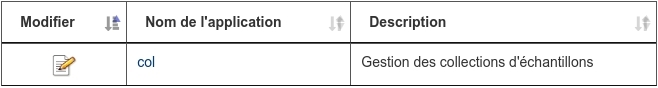
\includegraphics[width=\linewidth]{dessin/liste_appli}
\caption{Liste des applications déclarées}
\end{figure}

Pour créer une nouvelle application, choisissez \textit{Nouvelle application...}. 

\begin{figure}[H]
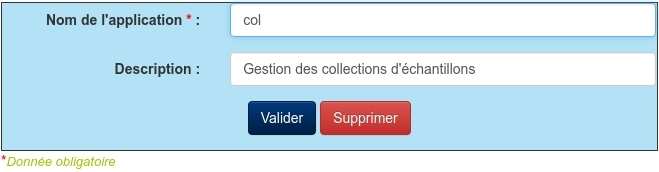
\includegraphics[width=\linewidth]{dessin/appli_change}
\caption{Écran de saisie d'une application}
\end{figure}

Le nom de l'application doit impérativement correspondre à la valeur \textit{\$GACL\_appli} dans les fichiers de paramètres : c'est ce qui permet au framework de savoir quels droits appliquer.

\subsection{Définir les droits utilisables dans l'application}

À partir de la liste des applications, cliquez sur le nom de celle pour laquelle vous voulez définir les droits utilisables. 
À partir de la liste, sélectionnez \textit{Nouveau droit...}.

\begin{figure}[H]
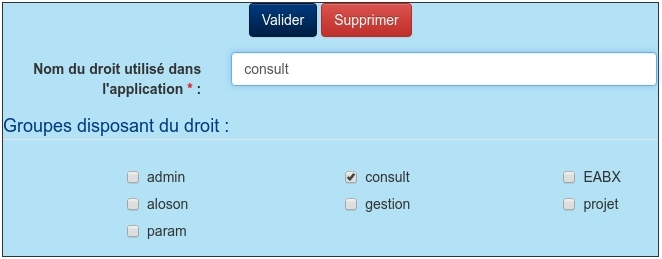
\includegraphics[width=\linewidth]{dessin/appli_droit}
\caption{Écran de saisie des droits associés à une application}
\end{figure}

Le nom du droit doit être celui défini dans le corps de l'application (les droits sont positionnés dans les fichiers \textit{param/actions.xml}, qui contient la liste des modules utilisables, et \textit{param/menu.xml}, qui sert à générer le menu).

Indiquez les groupes d'utilisateurs qui seront associés au droit courant.

\subsection{Désactiver la création de nouveaux droits}

En production, il peut être opportun de désactiver la création de nouveaux droits. Pour cela, il faut positionner à 1 la variable \textbf{GACL\_disable\_new\_right} dans le fichier \textit{param.default.inc.php} (ou \textit{param.inc.php}).

\subsection{Cas particulier des groupes et des logins issus d'un annuaire LDAP}

Si vous avez paramétré l'application pour qu'elle s'appuie sur un annuaire LDAP pour gérer l'affectation des utilisateurs dans les groupes, vous n'êtes pas obligés de les déclarer explicitement dans le module de gestion des droits.

\subsubsection{Droits attribués à un groupe LDAP}

Tous les utilisateurs d'un groupe héritent d'un droit dans l'application.

\begin{itemize}
\item définissez le nom du groupe (en respectant la casse) dans le tableau des groupes d'utilisateurs ;
\item sélectionnez le nom de ce groupe dans les droits utilisables ;
\item tous les utilisateurs de l'annuaire LDAP récupéreront automatiquement les droits attribués à ce groupe.
\end{itemize}

\subsubsection{Droits attribués à un utilisateur particulier de l'annuaire LDAP}

Un utilisateur s'identifie auprès de l'annuaire LDAP, mais dispose de droits particuliers.

\begin{itemize}
\item créez son login dans la gestion des droits ;
\item rajoutez-le dans le groupe d'utilisateurs adéquat.
\end{itemize}

\subsection{Pour mieux comprendre la gestion des droits}

Des vidéos ont été créées dans le cadre du logiciel Collec-Science\footnote{\href{https://www.collec-science.org}{https://www.collec-science.org}}) :
\begin{itemize}
\item \href{https://youtu.be/7NCNQuHoI8s}{https://youtu.be/7NCNQuHoI8s}
\item \href{https://youtu.be/j_iI8_g-u7w}{https://youtu.be/j\_iI8\_g-u7w}
\end{itemize}
